%%%%%%%%%%%%%%%%%%%%%%%%%%%%% Define Article %%%%%%%%%%%%%%%%%%%%%%%%%%%%%%%%%%
\documentclass[twocolumn]{article}
%%%%%%%%%%%%%%%%%%%%%%%%%%%%%%%%%%%%%%%%%%%%%%%%%%%%%%%%%%%%%%%%%%%%%%%%%%%%%%%

%%%%%%%%%%%%%%%%%%%%%%%%%%%%% Using Packages %%%%%%%%%%%%%%%%%%%%%%%%%%%%%%%%%%
\usepackage{geometry}
\usepackage{graphicx}
\usepackage{amssymb}
\usepackage{amsmath}
\usepackage{amsthm}
\usepackage{empheq}
\usepackage{mdframed}
\usepackage{booktabs}
\usepackage{lipsum}
\usepackage{graphicx}
\usepackage{color}
\usepackage{psfrag}
\usepackage{pgfplots}
\usepackage{bm}
% My packages
\usepackage{enumitem}
\usepackage[spanish]{babel}
\usepackage{placeins}

\usepackage{biblatex} 

\usepackage{hyperref}
%%%%%%%%%%%%%%%%%%%%%%%%%%%%%%%%%%%%%%%%%%%%%%%%%%%%%%%%%%%%%%%%%%%%%%%%%%%%%%%

% Other Settings
% Figures folder
\graphicspath{{Figures/}}


%%%%%%%%%%%%%%%%%%%%%%%%%% Page Setting %%%%%%%%%%%%%%%%%%%%%%%%%%%%%%%%%%%%%%%
\geometry{a4paper}

% my configuration
\setlist[enumerate]{label=\alph*)}

%%%%%%%%%%%%%%%%%%%%%%%%%%%%%%% Plotting Settings %%%%%%%%%%%%%%%%%%%%%%%%%%%%%
\usepgfplotslibrary{colorbrewer}
\pgfplotsset{width=8cm,compat=1.9}
%%%%%%%%%%%%%%%%%%%%%%%%%%%%%%%%%%%%%%%%%%%%%%%%%%%%%%%%%%%%%%%%%%%%%%%%%%%%%%%

%%%%%%%%%%%%%%%%%%%%%%%%%%%%%%% Title & Author %%%%%%%%%%%%%%%%%%%%%%%%%%%%%%%%
\title{Solución del átomo de Hidrógeno}
\author{Luis Daniel Díaz Durango}
\hypersetup{
    colorlinks=true,
    linkcolor=blue,
    filecolor=blue,      
    urlcolor=blue,
    citecolor=blue
    }
%%%%%%%%%%%%%%%%%%%%%%%%%%%%%%%%%%%%%%%%%%%%%%%%%%%%%%%%%%%%%%%%%%%%%%%%%%%%%%%

\begin{document}
\maketitle

Partamos de la ecuación diferencial que describe el átomo de Hidrógeno.

\begin{equation}
    \label{eq:Schrodinger}
    \left\{- \frac{\hbar^2}{2m} \nabla^2  - V(r)\right\} \psi = E \psi
\end{equation}

Sabemos que el proton y el electrón tienen cargas opuestas, por lo tanto, el potencial $V(r)$, que es el potencial de Coulomb, queda de la forma $V(r) = \frac{1}{4\pi \epsilon_0} \frac{q_1 q_2}{r} =- \frac{1}{4\pi \epsilon_0} \frac{e^2}{r} = -\frac{\alpha}{r}$, con $\alpha = \frac{e^2}{4\pi \epsilon_0}$. De modo que la ecuación queda de la forma:

\begin{equation}
    \label{eq:Schrodinger2}
    \left\{- \frac{\hbar^2}{2m} \nabla^2  - \frac{\alpha}{r}\right\} \psi = E \psi
\end{equation}

Una forma lógica de proceder, es escogiendo un sistema coordenado que simplifique las soluciones. En este caso, por ser un problema central, como observamos desde la forma del potencial $V(r)$, es conveniente usar coordenadas esféricas. El laplaciano en coordenadas esféricas es:

\begin{align*}
    \label{eq:Laplaciano}
    \nabla^2 \psi &= \frac{1}{r^2} \frac{\partial}{\partial r} \left(r^2 \frac{\partial \psi}{\partial r}\right) + \frac{1}{r^2 \sin \theta} \frac{\partial}{\partial \theta} \left(\sin \theta \frac{\partial \psi}{\partial \theta}\right) \\
    &+ \frac{1}{r^2 \sin^2 \theta} \frac{\partial^2 \psi}{\partial \phi^2}
\end{align*}

Por tanto, la ecuación de Schrödinger en coordenadas esféricas es:

\begin{align*}
    E\psi = 
    -\frac{\hbar^2}{2m} \frac{1}{r^2}
    \bigg\{
    & \frac{\partial}{\partial r} \left(r^2 \frac{\partial \psi}{\partial r}\right) 
    + \frac{1}{\sin \theta} \frac{\partial}{\partial \theta} \left(\sin \theta \frac{\partial \psi}{\partial \theta}\right) \\ 
    &+ \frac{1}{\sin^2 \theta} \frac{\partial^2 \psi}{\partial \phi^2}\bigg\} - \frac{\alpha}{r}\psi
\end{align*}

Así, podemos hacer separación de variables, esto es, $\psi(r, \theta, \phi) = R(r) T(\theta) P(\phi)$, Así, multiplicando por $r^2/\psi$, y organizando los términos por variables:

\begin{align*}
    Er^2 = &-\frac{\hbar^2}{2m} \left\{ \frac{r^2}{R} \frac{d^2R}{dr^2} + \frac{2r}{R} \frac{dR}{dr} \right\} - \alpha r \\
    &- \frac{\hbar^2}{2m} \left\{ \frac{1}{T\sin \theta} \frac{d}{d \theta } \left(\sin \theta \frac{d T}{d \theta}\right) \right\} \\
    &- \frac{1}{P\sin^2 \theta} \frac{d^2 P}{d \phi^2}
\end{align*}

Por la periodicidad en la variable $\phi$, está claro que la solución de $P(\phi)$ tiene que ser senos y cosenos, y para $\theta$, la solución son los polinomios asociados de Legendre, por lo que el producto de estas corresponde a los armónicos esféricos. Por otra parte, la solución a la parte radial corresponde a los polinomios de Laguerre. Así, la solución general es:

\begin{equation}
    \label{eq:Solucion}
    \psi_{nlm} = R_{nl}(r) Y_{lm}(\theta, \phi)
\end{equation}

A continuación se muestran gráficas de los primeros armónicos esféricos con m=0.

\begin{figure}[h!]
    \caption{l=0, m=0}
    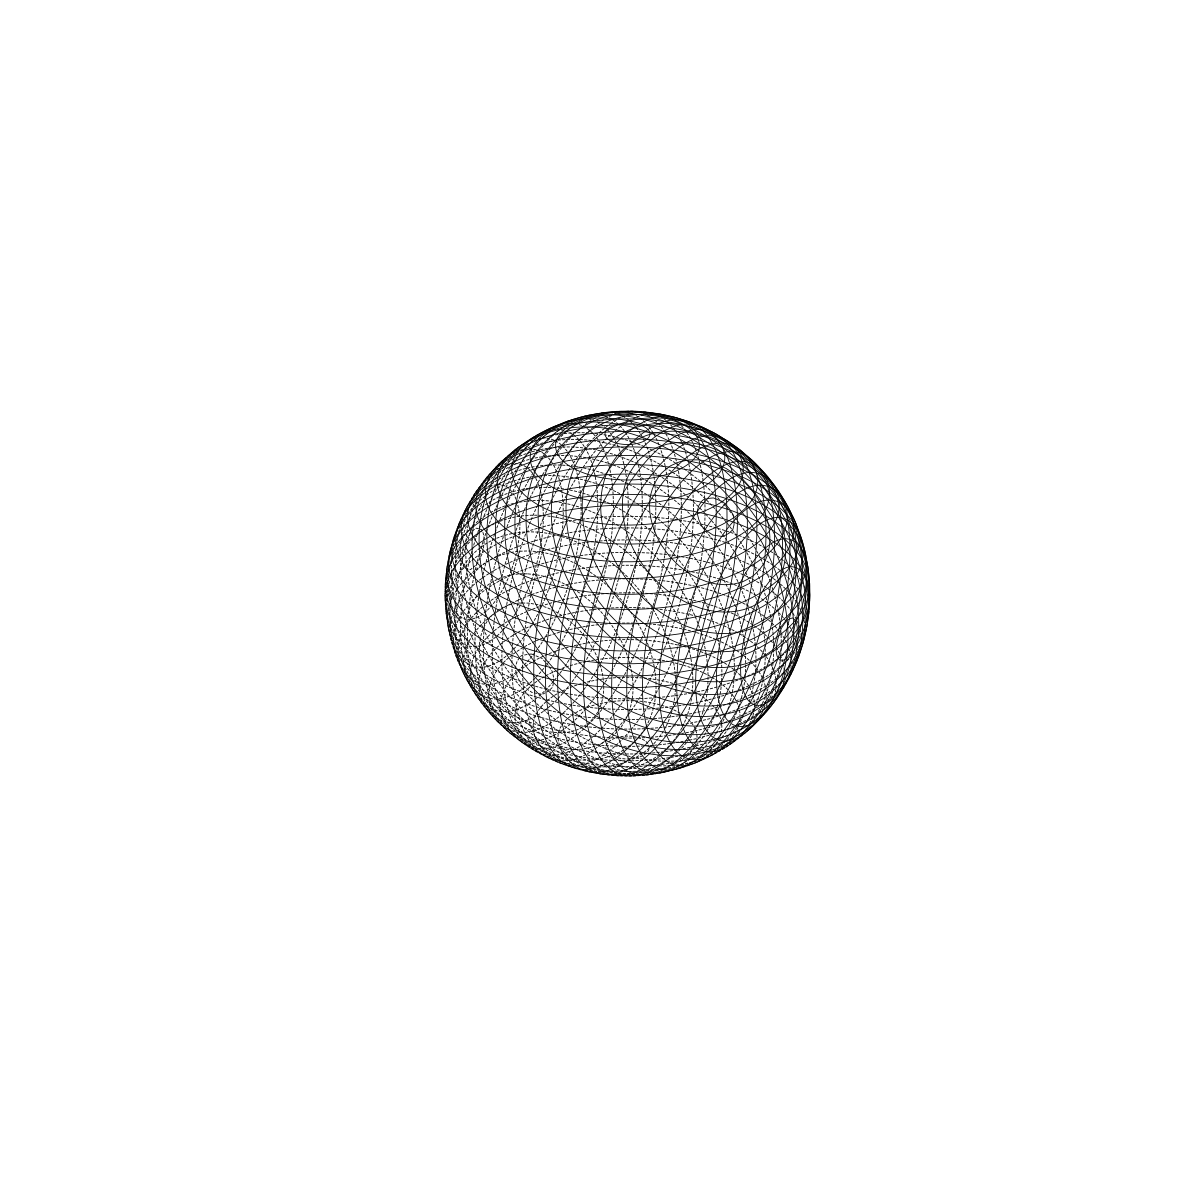
\includegraphics[width=0.5\textwidth]{Y0-0.png}    
\end{figure}

\begin{figure}[h!]
    \caption{l=1, m=0}
    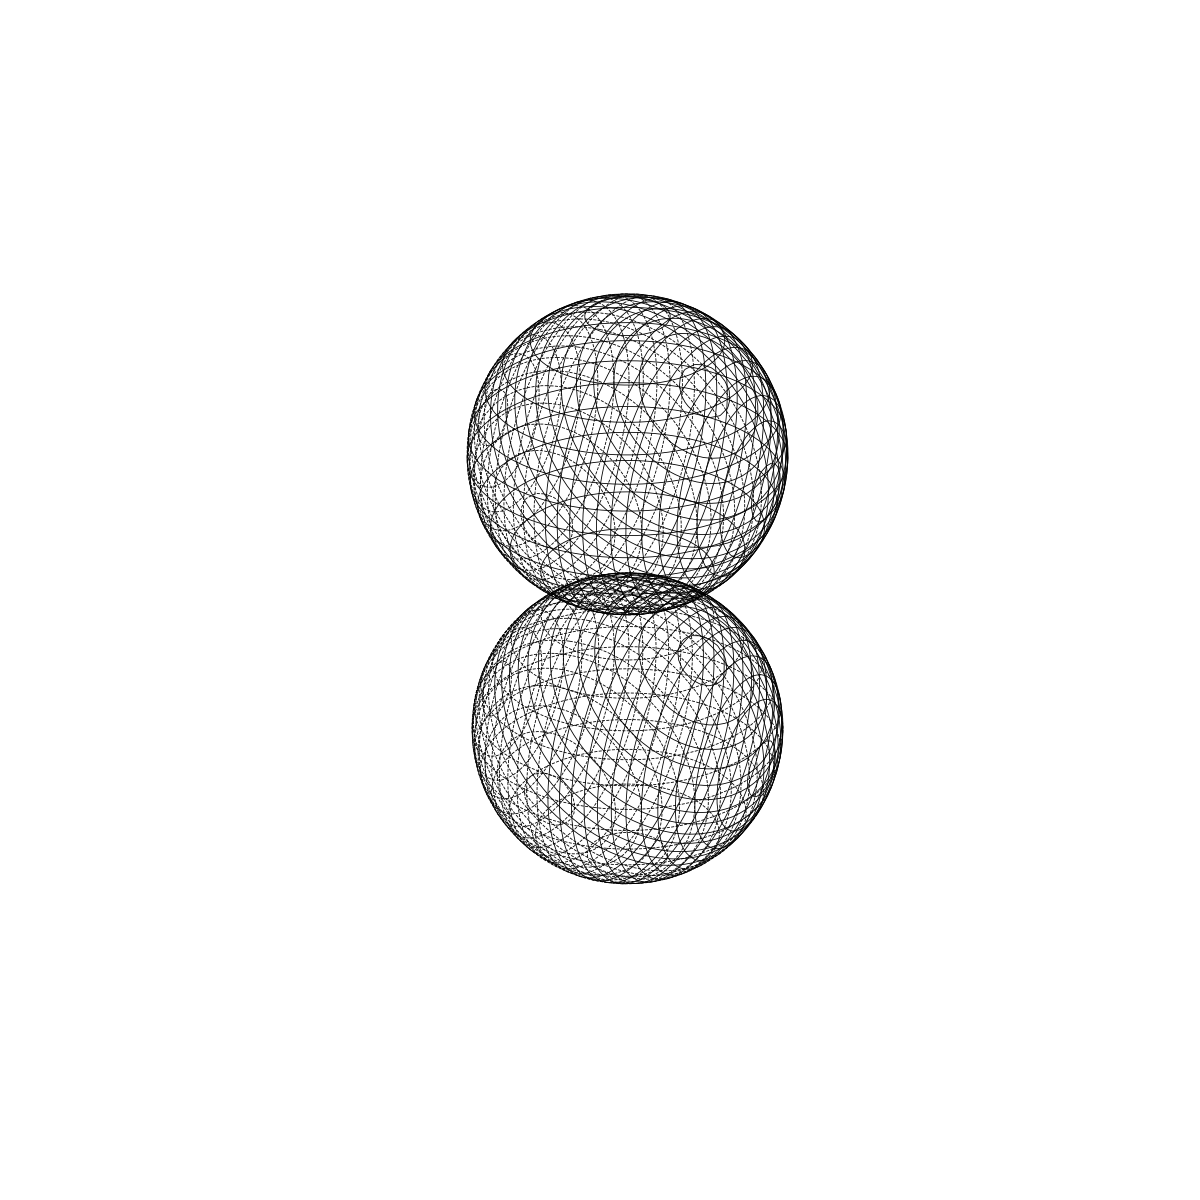
\includegraphics[width=0.5\textwidth]{Y1-0.png}    
\end{figure}

\begin{figure}[h!]
    \caption{l=2, m=0}
    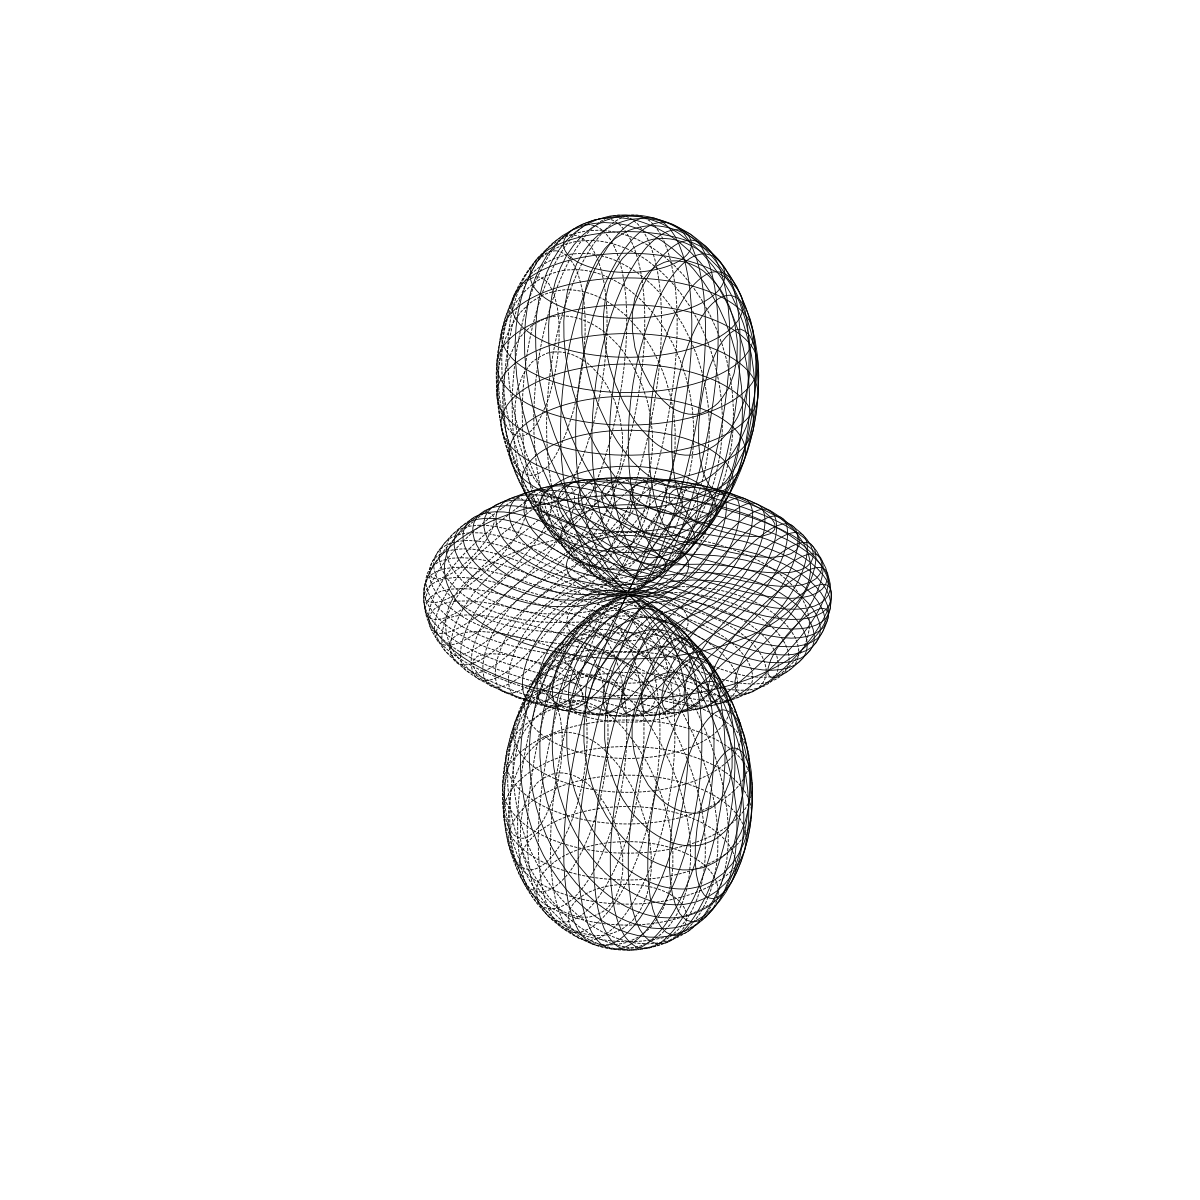
\includegraphics[width=0.5\textwidth]{Y2-0.png}
\end{figure}

\begin{figure}[h!]
    \caption{l=3, m=0}
    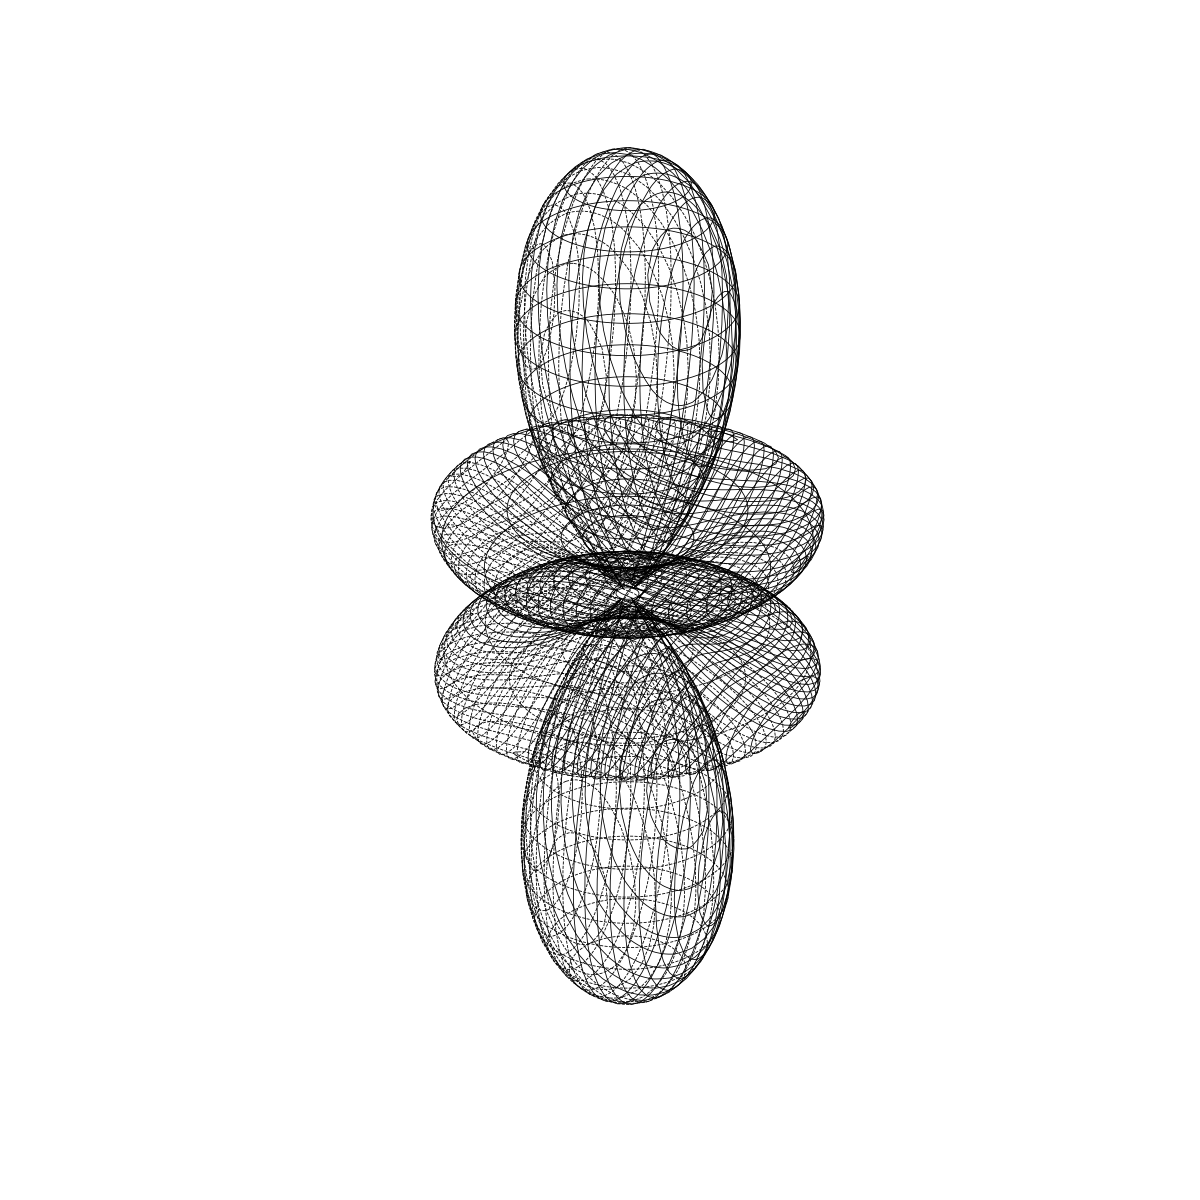
\includegraphics[width=0.5\textwidth]{Y3-0.png}
\end{figure}


Con este \href{https://github.com/lldddv2/Atomo_de_Hidrogeno}{link}, se puede acceder al código fuente de este documento, al pdf generado, y el código fuente de las gráficas.

\end{document}